\section{Partie théorique -- Exercices}
\noindent Soit l'image RGB de 8 pixels suivante :

\vspace{0.2cm}
\noindent
\begin{minipage}[c]{\textwidth}
  \centering
  \makebox[\textwidth]{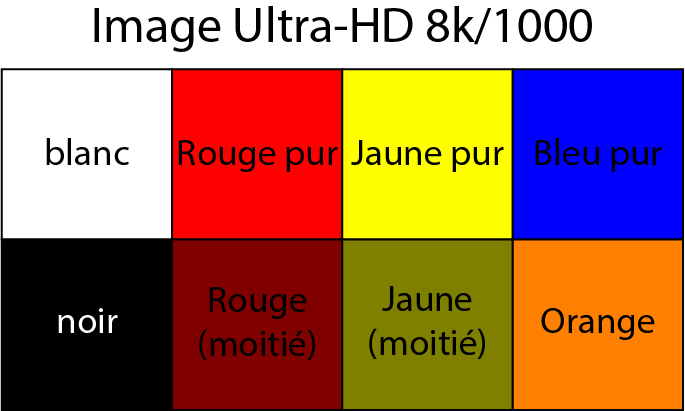
\includegraphics[width=\linewidth]{addOns/Image8K.png}}\\
  \captionof{figure}{Image 8 pixels}
  \label{fig.Image_UHD_8K}
\end{minipage}\\


\subsection{Isoler le canal rouge}
En imaginant que vous vouliez analyser la composante Rouge de l'image ~\ref{fig.Image_UHD_8K} -- soit l'intensité lumineuse rouge pour chacun des pixels de l'image :

\vspace{0.2cm}
\noindent \textbf{Quelles sont alors les valeurs (théoriques) des canaux que vous vous attendez à observer ?} (Remplissez le tableau ci-dessous)

\vspace{0.2cm}
\begin{table}[ht]
  \renewcommand{\arraystretch}{3}
  \newcolumntype{x}[1]{>{\centering\let\newline\\\arraybackslash\hspace{0pt}}p{#1}}
  \center
  \begin{tabular}{|x{3cm}|x{3cm}|x{3cm}|x{3cm}|x{3cm}|}
    \hline
    & & & \\
    \hline
    & & &\\
    \hline
  \end{tabular}
\end{table}

\vspace{0.2cm}

\noindent \textbf{Quelles opérations appliquer à l'image d'entrée pour en obtenir ces informations ?}

\vspace{4cm}


\subsection{Extraire la couleur rouge}
En imaginant maintenant que vous ne vouliez obtenir non plus une image qui contient toute l'information de rouge de l'image, mais une image n'a de pixels allumés en nuance de gris \textbf{qu'aux endroits où les pixels sont rouges dans l'image d'entrée}.

\vspace{0.2cm}
\noindent\textbf{Quelles sont alors les valeurs (théoriques) des pixels que vous vous attendez à observer ?} (Remplissez le tableau ci-dessous)

\vspace{0.2cm}
\begin{table}[ht]
  \renewcommand{\arraystretch}{3}
  \newcolumntype{x}[1]{>{\centering\let\newline\\\arraybackslash\hspace{0pt}}p{#1}}
  \center
  \begin{tabular}{|x{3cm}|x{3cm}|x{3cm}|x{3cm}|x{3cm}|}
    \hline
    & & & \\
    \hline
    & & &\\
    \hline
  \end{tabular}
\end{table}

\vspace{0.2cm}

\noindent \textbf{Quelles opérations appliquer à l'image d'entrée pour en obtenir ces informations ?}

\vspace{4cm}


\subsection{Extraire la couleur jaune}
\noindent Même problème, mais pour la couleur jaune :

\vspace{0.2cm}
\noindent \textbf{Quelles sont alors les valeurs (théoriques) des pixels que vous vous attendez à observer ?} (Remplissez le tableau ci-dessous)

\vspace{0.2cm}
\begin{table}[ht]
  \renewcommand{\arraystretch}{3}
  \newcolumntype{x}[1]{>{\centering\let\newline\\\arraybackslash\hspace{0pt}}p{#1}}
  \center
  \begin{tabular}{|x{3cm}|x{3cm}|x{3cm}|x{3cm}|x{3cm}|}
    \hline
    & & & \\
    \hline
    & & &\\
    \hline
  \end{tabular}
\end{table}

\vspace{0.2cm}

\noindent \textbf{Quelles opérations appliquer à l'image d'entrée pour en obtenir ces informations ?}

\vspace{4cm}


\subsection{Extraire la couleur orange}
\noindent Même problème, mais pour la couleur orange :

\vspace{0.2cm}
\noindent \textbf{Quelles sont alors les valeurs (théoriques) des pixels que vous vous attendez à observer ?} (Remplissez le tableau ci-dessous)

\vspace{0.2cm}
\begin{table}[ht]
  \renewcommand{\arraystretch}{3}
  \newcolumntype{x}[1]{>{\centering\let\newline\\\arraybackslash\hspace{0pt}}p{#1}}
  \center
  \begin{tabular}{|x{3cm}|x{3cm}|x{3cm}|x{3cm}|x{3cm}|}
    \hline
    & & & \\
    \hline
    & & &\\
    \hline
  \end{tabular}
\end{table}

\vspace{0.2cm}

\noindent \textbf{Quelles opérations appliquer à l'image d'entrée pour en obtenir ces informations ?}

\vspace{4cm}